\documentclass[a4paper,11pt]{article}
\usepackage[margin=3cm]{geometry}
\linespread{1.25}

\usepackage[T1]{fontenc}
\usepackage[utf8]{inputenc}
% \usepackage[swedish]{babel}
% \usepackage{fontspec}
% \setmainfont{Linux Libertine O}
\usepackage{lmodern}
\usepackage{graphicx}
\usepackage{float}
\usepackage{subfig}
\usepackage{hyperref}
\usepackage{pdfpages}

\usepackage{fancyhdr}
\pagestyle{fancy}
\renewcommand{\headrulewidth}{ 1.0pt }
\renewcommand{\footrulewidth}{ 0.4pt }
\fancyhead{} % clear all headers
\fancyfoot{} % clear all footers

% E:even page, O:odd page, L:left, C:center, R:right
%\fancyhead[LE,RO]{\thepage}
%\fancyfoot[C]  {Albert Einstein, 2009}

\fancyhead[L]{DH2323 (DGI17) Raytracer Project Report}
\fancyhead[R]{Mikael Forsberg, Robin Gunning}
\fancyfoot[C]{\thepage}

\begin{document}
\pagenumbering{gobble}
\title{\vspace{-1cm} \Huge Raytracer Project Report\\ \large DH2323 (DGI17)\\ KTH Royal Institute of Technology}
\author{Mikael Forsberg <miforsb@kth.se>\\ Robin Gunning <rgunning@kth.se>}
\maketitle

\newpage
\tableofcontents
\newpage
\pagenumbering{arabic}

\section{Preface: abbreviated project specification}
This sections contains an abbreviated version of the project specification that we submitted
on May 3rd.
\vspace{-0.3cm}
\subsection{Idea}
\vspace{-0.3cm}
The idea of the project is to explore more features common in ray tracing rendering
in an effort to gain an increased understanding of conventional ray tracing in general.
We will do this by adding a number of features to the baseline feature set defined by
the ray tracer implemented in lab 2.

\subsection{Project plan}
\vspace{-0.3cm}
The following section contains two sets of implementation goals. The first set (''Baseline'')
is what we consider to be the minimum for project completion, while the second set (''Bonus'')
contains ideas that are not essential but could improve the project should we find the time to
implement them.

\subsection{Baseline features}
\vspace{-0.3cm}
\noindent \textbf{Fast wireframe view}\\
The application should default to a wireframe renderer. From the wireframe mode the user
should be able to initiate a single-frame high-quality render or simply a switch to continuous
ray tracing, as well as be able to switch back to wireframe.

\noindent \textbf{Multithreading}\\
Rendering should be parallelized by partitioning the screen space and rendering
each part in a separate thread. The number of threads should be configurable.

\noindent \textbf{Back-face culling}

\noindent \textbf{Loading of models in the \texttt{.STL}\footnote{\url{https://en.wikipedia.org/wiki/STL\_(file\_format)}} format}

\noindent \textbf{Loading of models in the Wavefront \texttt{.OBJ}\footnote{\url{http://www.martinreddy.net/gfx/3d/OBJ.spec}} format}\\
Features supported by the format that are outside the scope of basic triangle geometry (free-form
curves, smoothing groups etc.) are not part of this goal.

\noindent \textbf{Phong interpolation and the Phong reflection model}

\noindent \textbf{Materials}\\
Primitives such as triangles should support being assigned a ''material''.
The following properties should be implemented:
\vspace{-.3cm}

\begin{itemize}
\item[]\noindent \hspace{-.5cm} • \textbf{Phong properties (colors for ambient, specular, diffuse)}
\vspace{-.2cm}

\noindent \hspace{-.5cm} • \textbf{Texture mapping}
\vspace{-.2cm}

\noindent \hspace{-.5cm} • \textbf{Opacity}
\vspace{-.2cm}

\noindent \hspace{-.5cm} • \textbf{Specular reflection and reflectivity}
\vspace{-.2cm}

\noindent \hspace{-.5cm} • \textbf{Refraction}
\end{itemize}

\noindent \textbf{Non-triangle based primitives: Spheres}\\
The ray tracer should support rendering perfect spheres defined by position and radius.
Spheres should support the same material settings as other primitives and should also be
shown appropriately in the wireframe view.

\noindent \textbf{Area lights and soft shadows}\\
We will attempt to implement soft shadows by some method of simulating area lights (as
opposed to the point light simulated in the labs).

\subsection{Bonus features}
\vspace{-.3cm}
\begin{itemize}
\item[•] \textbf{Support the \texttt{.MTL} format as companion to \texttt{.OBJ}}
\vspace{-0.3cm}
\item[•] \textbf{Anti-aliasing}
\vspace{-0.3cm}
\item[•] \textbf{Fast flat-shaded view}
\vspace{-0.3cm}
\item[•] \textbf{Normal mapping}
\end{itemize}

\subsection{Implementation}
The features will be implemented in a single executable application using C++ and SDL2.

\subsection{Evaluation}
The final application could be evaluated by comparing images created with other renderers to
images created with our application. There are atleast a few commonly used
scenes and objects (the Cornell box, the Stanford bunny) available for such comparisons.

\section{Blog}
Here is a link to our blog: \url{https://dybtracer.blogspot.se/}

\newpage
\section{Implementation}
This section describes the work that has been done. The section
begins with a short summary of the overall result followed by a short overview of the design
of the code. We then go through the individual feature goals as defined by the project
specification and describe implementation details along with notes on major problems and
their solutions. Finally, the section ends with a short discussion on any planned features
that where not implemented.

\subsection{Summary}
All baseline features except area lights were implemented. None of the bonus features
mentioned in the specification were implemented. Three bonus features not mentioned
in the specification have been implemented (bounding volume hierachies, metallic reflections
and Lua scripting).

\subsection{Design overview}
The overall design is based on the simple pattern of concrete objects being used via
a layer of interface abstraction. The most important interfaces and their implementations
are listed below, along with one or two central methods of each interface:
\vspace{0.3cm}

\begin{tabular}{l l l}
\textbf{Interface} & \textbf{Method(s)} & \textbf{Implementation(s)}\\
\hline
\texttt{PixelSurface} & \texttt{setPixel(x, y, r, g, b)} & \texttt{SDLGui}\\
\hline
\texttt{GUI} & \texttt{createWindow(title, w, h)} & \texttt{SDLGui}\\
    & \texttt{getEvents(vector\&)} & \\
\hline
\texttt{Texture} & \texttt{getColorAt(coords)} & \texttt{SDLTexture}\\
\hline
% FileDialog & GtkFileDialog\\ % not important
\texttt{Object} & \texttt{getIntersection(from,dir,Intersection\&)} & \texttt{Mesh}, \texttt{Sphere}\\
& \texttt{getWireframe(vector\&)} & \\
\hline
\texttt{Renderer} & \texttt{renderScene(scene, w, h, PixelSurface\&)} & \texttt{WireframeRenderer},\\
         & & \texttt{RayTracingRenderer}
\end{tabular}
\vspace{0.5cm}

\noindent
The pattern is then implemented throughout the code by having as much code as possible
depend on the interfaces instead of the concrete classes. As an example, neither
\texttt{WireframeRenderer} nor \texttt{RayTracingRenderer} knows anything about the specifics of the existing
concrete objects (\texttt{Mesh} and \texttt{Sphere}) beyond what is exposed by the \texttt{Object} interface.

There are however several compromises to the pattern present in the current code. One example
being the \texttt{SDLGui} class exposing a method \texttt{saveBMP} that is not part of the \texttt{GUI} interface, which
means the client code using this method is tightly coupled to the \texttt{SDLGui} class.
There are also several classes/structures that currently do not use an interface
abstraction at all, such as \texttt{Intersection}, \texttt{Material} and \texttt{Light}.

\subsection{Implemented baseline features}
\subsubsection{Switchable renderers}
Switchable renderers were implemented by making use of the \texttt{Renderer} interface abstraction.
The main application uses three pointers to instances of \texttt{Renderer}, two of which are initiated
by constructing one \texttt{WireframeRenderer} and one \texttt{RayTracingRenderer}. The third pointer is
the ''active'' renderer, and is always set to equal one of the other pointers. Keyboard
buttons are used to toggle the active renderer between the two possible values, where one
button (R) is used to simply switch between renderers, and another button (T) is used to
raytrace a single frame by switching specifically to the raytracing renderer and setting
a flag to disable rendering until T is pressed a second time. While rendering is disabled
the GUI will draw the last rendered frame repeatedly.

\begin{figure}[H]
    \centering
    \subfloat[Wireframe mode]{{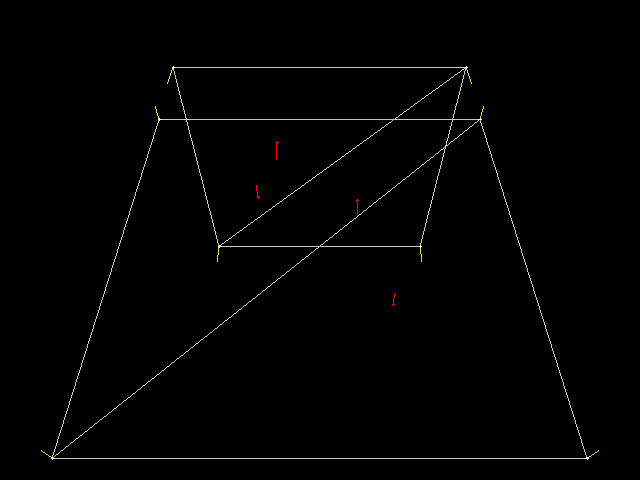
\includegraphics[width=5cm]{mode-wire.png} }}
    \qquad
    \subfloat[Raytracing mode]{{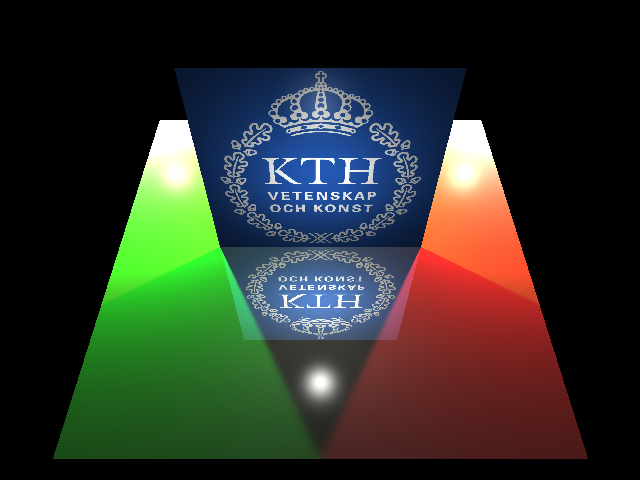
\includegraphics[width=5cm]{mode-ray.png} }}
    \caption{Switchable renderer}
\end{figure}

\subsubsection{Multithreading}
Multithreading was surprisingly straightforward to implement despite never having done
multithreading in C/C++ before. Multithreading is only implemented for the raytracer and
consists the \texttt{renderScene} method setting up a number of threads that each run the
private \texttt{renderingThread} method. Each thread has access to a pthread \texttt{thread\_data} structure
in which we store the screen space bounds ($x_{from},\; x_{to},\; y_{from},\; y_{to}$) for the
thread in question. The screen space is partitioned by setting different screen space bounds
for each thread. There is also a progress counter implemented using a counter protected
by a mutex. The progress counter simply reports the number of horizontal lines
that have been completed.

At the moment, the screen is partitioned in full-width horizontal parts. This
is not ideal since it often leads to large differences in workloads for different threads. As an
example, picture rendering a complex model of a car sitting on a simple floor or in a void.
The camera will probably be positioned so as to place the car more or less centered in frame
with some room above and below it so the resulting image does not become cramped. This means
that the first and last threads in particular will have a very small workload compared to
threads that handle the areas closer to the center of the screen space, simply because most
rays in the first and last threads will not intersect with the car model at all. The result
of having unbalanced workloads is that some threads will exit early while others are still
processing, often ending in a situation where the CPU becomes under-utilized because there
are not enough active threads, making the rendering take longer to complete. With the progress
counter enabled, the effect can be seen as progress slows down towards the end of the
rendering.

The performance increase can be seen in a demo video we created for the blog:

\begin{center}\url{https://www.youtube.com/watch?v=u2EZAErKC1c}\end{center}

The machine used in the demo has two physical cores and four logical cores, and as shown
in the video the performance scales close to linearly going from one to two threads while not
giving any substantial gains when the thread count is further increased.

\subsubsection{Backface culling}
% TODO: (maybe) add something on problems with vertex order
We implemented the simplest possible form of backface culling in \texttt{Mesh::cullInvisibleParts}.
The method takes the current position of the camera and sets a ''hidden'' flag on every
triangle for which the angle between the surface normal of the triangle and a vector
from the the first vertex of the triangle to the camera position is larger than 90 degrees.

We had an issue with backface culling which in retrospect appears completely obvious.
Backface culling was implemented before Phong interpolation. At that point, all vertex
normals of all triangles were set to the triangle surface normal as computed by cross product
on two edges of the triangle. After implementing Phong interpolation and using real, individual
vertex normals on triangles the backface culling started behaving incorrectly, culling 
triangles that should not be culled. This is of course due to vertex normals rarely aligning
with the surface normal as was expected by the backface culling code. The solution was 
to add storage of the computed cross product surface normal in each triangle and have the
backface culling code use it.

Unfortunately, backface culling does not play nice with reflections without changing which faces
are currently culled for each reflected ray. The fact that we render using several parallel
threads means that fixing this is not entirely trivial, and so backface culling has been disabled
in the code.

\begin{figure}[H]
\begin{center}
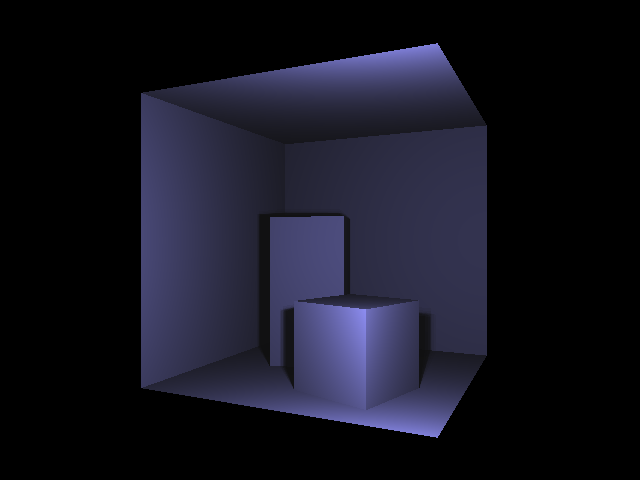
\includegraphics[width=5.5cm]{bfcull.png}
\caption{Culled wall in Cornell box}
\end{center}
\end{figure}
\vspace{-0.5cm}

\subsubsection{Loading .OBJ files}
Mikael had written an \texttt{.OBJ} parser/loader while experimenting with lab 3 where it simply
dumped triangles into a provided \texttt{vector<Triangle>} reference. Changing this code to instead generate a
\texttt{Mesh} object was trivial. After Phong interpolation had been implemented the \texttt{.OBJ} parser was
extended with the ability to read vertex normal entries as it had previously only cared
about vertex and face entries.

\begin{figure}[H]
\begin{center}
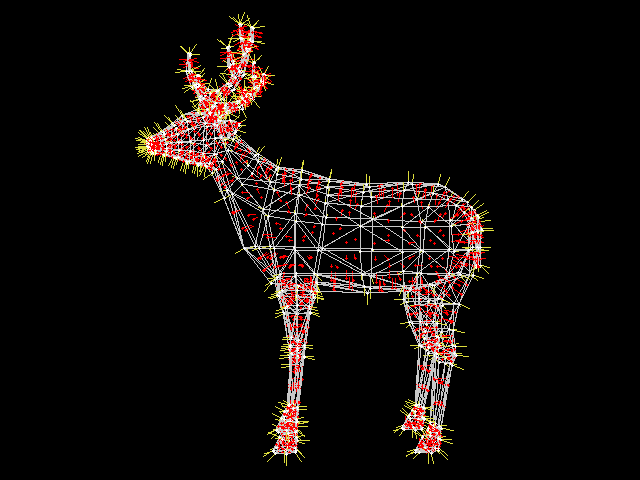
\includegraphics[width=5.5cm]{obj-deer.png}
\caption{Geometry and normals loaded from an .OBJ file}
\end{center}
\end{figure}
\vspace{-0.5cm}

\subsubsection{Loading .STL files}
We decided only to implement the binary version of the \texttt{.STL} format since the plain text version
is an older version which takes up more space and is rarely used. Luckily there was pretty detailed
information on how binary \texttt{.STL} files are represented on
Wikipedia\footnote{\url{https://en.wikipedia.org/wiki/STL\_(file\_format)\#Binary\_STL}}.

% The first 80 bytes contains the header for the model (modelname or author).
% The next 32 bits contains the number of total triangles in the model.
% For every triangle there are 3*4 bytes containing the normal vectors of the triangle, 
% 3*(3*4 bytes information about the position of the vertex) and lastly there are 2 bytes of
% attribute byte count which is 0 in the standard format.

% STL file format is a very popular format for the 3d-printing community since it's using triangles 
% only, which makes it easy to translate into code for the 3d-printer to print.
% STL files can be either in plain text or in binary. 

\subsubsection{Phong interpolation}
Phong interpolation was implemented in the \texttt{Mesh} class by computing barycentric coordinates for 
a point of intersection and using these as weighting for combining the three vertex normals.
The code for barycentric coordinate computation was found on
StackExchange\footnote{\url{https://gamedev.stackexchange.com/a/23745}} where the post in question
references the book Real-Time Collision Detection by Christer Ericson.

The research and addition of barycentric coordinate computation had actually been done for
reasons of texture mapping, and so it was a happy discovery to be able to do the interpolation
of normals without needing any new maths.

\begin{figure}[H]
    \centering
    \subfloat[No interpolation]{{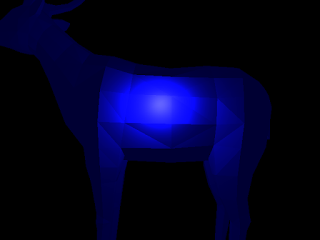
\includegraphics[width=5cm]{phong-none.png} }}
    \qquad
    \subfloat[Phong interpolation]{{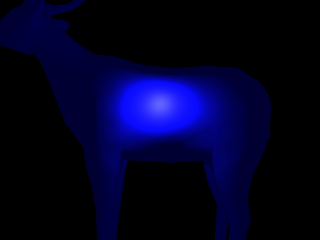
\includegraphics[width=5cm]{phong-interpolation.png} }}
    \caption{Phong interpolation}
\end{figure}

\subsubsection{Phong reflection model}
The Phong reflection model was implemented using the exact formula as presented on
Wikipedia\footnote{\url{https://en.wikipedia.org/wiki/Phong\_reflection\_model\#Description}}.
Since the formula accounts for multiple light sources, this turned out to be an opportune
time to implement support for multiple lights in the \texttt{Scene} class. Furthermore, the
''Phong parameters'' ($k_s,\; k_d,\; k_a$ and $\alpha$ for specular, diffuse, ambient colors
and shininess, respectively) were added to the \texttt{Material} structure at this time.

\begin{figure}[H]
\begin{center}
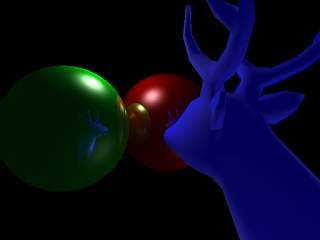
\includegraphics[width=5.5cm]{phong-reflections-demo.png}
\caption{Phong reflection model with two lights}
\end{center}
\end{figure}
\vspace{-0.5cm}

\subsubsection{Materials}
\subsubsection{Texture mapping}
Texture mapping was implemented by introducing three new properties for ambient texture,
diffuse texture and specular texture to the \texttt{Material} structure, each holding a pointer to an
instance of the \texttt{Texture} interface which exposes the method \texttt{getColorAt(vec2 texturecoords)}.
Texture coordinates are computed as part of intersection testing in the object classes
(\texttt{Mesh} and \texttt{Sphere}). For triangle meshes, texture coordinates of
individual triangles are computed by combining the texture coordinate vectors of the vertexes
weighted by the barycentric coordinates of the point of intersection. It is currently
only possible to apply texture mapping to a mesh where the texture coordinates for each vertex
have been set in advance. For spheres, texture coordinates are computed using a formula found
on Wikipedia\footnote{\url{https://en.wikipedia.org/wiki/UV\_mapping\#Finding\_UV\_on\_a\_sphere}}.

We had actually not considered the implications of using the Phong
reflection model before starting our implementation of texture mapping. There was
initially some confusion as to which color component(s) (ambient, specular and diffuse) should
be replaced when a texture was present. The decision to have a separate texture slot for each color component came
pretty quickly, and we also decided to let the base color components act as weights on the
texture colors instead of just having texture colors replace the base colors.

In the current version of the raytracer we begin by taking copies of the base colors of the
material before checking if the material has any textures set. We then check each texture
pointer in turn, and for any that are set we multiply our copied color component by the
color we get from the texture. This introduces a couple of extra branches to the raytracing
code which is not a good thing from a performance perspective. A possible improvement to 
this will be discussed later in this document.

\begin{figure}[H]
\begin{center}
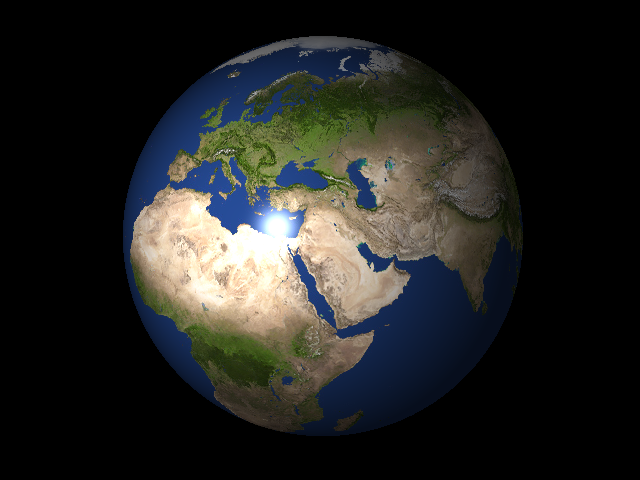
\includegraphics[width=5.5cm]{texmap-earth.png}
\caption{Texture mapping on a sphere}
\end{center}
\end{figure}
\vspace{-0.5cm}

\subsubsection{Opacity}
Opacity was initially implemented by equipping the \texttt{Material} structure with a single \texttt{float}
property for specifying opacity in the range of $[0,1]$. The effect was then simulated in
the raytracer. When a semitransparent material is hit, a new ray is cast from the point of
intersection of the original ray in the same direction as the original ray, collecting the
color from behind the semitransparent material and then mixing the two colors (the ''color
yonder'' and the color of the material itself) according to the opacity value.

Later in the project timeline we decided to change the opacity property (as well as the
reflection property, see below) to be per-component instead, going against the specification
slightly. The opacity property was therefore changed from a \texttt{float} to a \texttt{vec3}, giving more
flexibility to the material system.

\begin{figure}[H]
\begin{center}
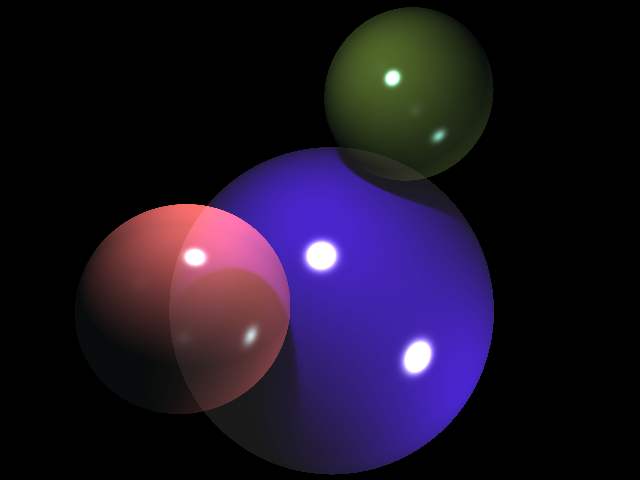
\includegraphics[width=5.5cm]{opac.png}
\caption{Opacity}
\end{center}
\end{figure}
\vspace{-0.5cm}

\subsubsection{Specular reflection}
% TODO: (maybe) something on the wacky first version of reflection
Mirror-like specular reflections were implemented in much the same way as opacity. The
\texttt{Material} structure was equipped with a float property for specifying reflectivity in the
range of $[0,1]$ and the effect was added to the raytracer. Just like for opacity, when a
reflective material is hit, a new ray is cast from the point of intersection of the original
ray, but this time the new ray is given a new direction according to the law of reflection.
The code for vector calculation of the new direction is heavily inspired by an
article\footnote{\url{http://www.3dkingdoms.com/weekly/weekly.php?a=2}} found on the website
3dkingdoms.com.

As noted in the specification there is an obvious risk of infinite loops here. To avoid
this problem, we introduced a \texttt{rayGeneration} counter parameter to the raycasting function
along with an immediate function return when this value grows too large. Each recursive
raycasting call simply adds one to the current generation value.

\begin{figure}[H]
\begin{center}
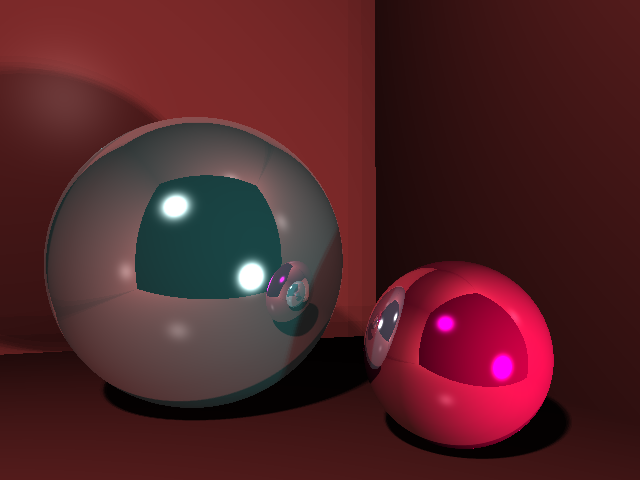
\includegraphics[width=5.5cm]{reflect.png}
\caption{A couple of reflective spheres in a box}
\end{center}
\end{figure}
\vspace{-0.5cm}

\subsubsection{Refraction}
Refraction was implemented by introducing a new property for the \texttt{Material} structure called \texttt{refraction}.
Standard refraction is used if no refraction has been set for the material and the standard 
refraction is set to 1 which is the refractive index for vacuum. 
Using Snell's law we cast a new refracted ray in the refracted direction coming out of the transparent material.

The refraction is represented as a \texttt{float} containing the refractive index of the material.
Since refraction isn't something we see and think about every day it's kind of hard to evaluate if
the refraction is realistic or not.%However i think it looks realistic for glass at the time being.

\subsubsection{Spheres}
Ray-sphere intersection testing was implemented using the ''analytic solution'' as presented
by Scratch-a-Pixel\footnote{\url{https://www.scratchapixel.com/lessons/3d-basic-rendering/minimal-ray-tracer-rendering-simple-shapes/ray-sphere-intersection}}
which consists of constructing and solving a quadratic equation. Spherical texture coordinates
are covered in section 2.3.9 on texture mapping.

The original plan for rendering spheres in wireframe view involved drawing curved lines, but
due to time constraints we opted for the simpler method of rough approximation by a set
of points interconnected by straight lines. The code still contains the framework support for
the original idea. The wireframe renderer collects a list of \texttt{WireframeElement} objects, each
containing a set of points along with normals for each of the points and an indicator for which kind of
''connector'' function is to be used for drawing the connecting lines. At this time the only
available connector is \texttt{Linear} which as the name implies performs linear interpolation
between points and thus draws straight lines.

\subsubsection{Soft shadows}
A very basic variant of soft shadows was implemented by casting additional, slightly perturbed
rays when doing the intersection test for shadows. Each of these $N$ rays then contribute
$1/N$ to a ''shadow factor'' value that is later multiplied with the lighting as computed by
the Phong model. The effect is definitely an improvement on single-ray hard shadows, but is
clearly not a particularly good solution as there is often visible color stepping in the
penumbra even at expensive (in terms of rendering time) ray counts.

Sadly we did not manage to spend nearly as much time on soft shadows as we had planned.
Area lights were sadly not implemented at all, and so the soft shadows really are just
a trick, not taking the geometry of the light source into account at all.

\subsection{Implemented bonus features}
None of the bonus features mentioned in the specification were implemented, but three
previously unmentioned features did make it into the project. These features are described
below along with some justification on why they were implemented.

\subsubsection{Bounding volume hierarchy optimization for ray-mesh intersection}
The \texttt{Mesh} class has been equipped with the ability to calculate a bounding box for its entire
set of triangles and then recursively subdivide this box into a hierarchy of smaller and
smaller bounding boxes, each box containing a list of pointers to the
triangles that intersect it along with pointers to its two sub-boxes. The triangle-box intersection
code\footnote{\url{http://fileadmin.cs.lth.se/cs/personal/tomas_akenine-moller/code/tribox3.txt}}
was published by Tomas Akenine-Möller on his website where he has also published a
paper\footnote{\url{http://fileadmin.cs.lth.se/cs/personal/tomas_akenine-moller/code/tribox\_tam.pdf}}
on his algorithm, which is based on the separating axis
theorem\footnote{\url{https://en.wikipedia.org/wiki/Hyperplane\_separation\_theorem}}. The
subdivision of a particular box is canceled if the depth of recursion exceeds a set limit
(5 in current version) or if the box does not contain enough triangles (minimum of 25 in
current version). Empty boxes are deleted and their pointer in their parent box is set
to nullptr.

This structure of boxes is then used to reduce the number of triangles that need to be tested
for intersection by only testing those triangles that are contained in boxes at the deepest
level that are intersected by a particular ray. The ray-box intersection code used was published
by Tavian Barnes at his blog on tavianator.com\footnote{\url{https://tavianator.com/fast-branchless-raybounding-box-intersections/}}.
Each box provides the guarantee that any triangle contained within it is also contained in one or
both of its sub-boxes, should they exist. As such, when testing for ray intersection, if the current
box has any sub-boxes it is safe to delegate intersection testing to them. In many cases, even if
the box has two sub-boxes that contain triangles, the current ray will only intersect one of them,
which means the triangles that are only contained in the other sub-box will not be tested for intersection.

The increase in performance is substantial. When rendering the following, reasonable
(as in an image someone might realistically want to render) image of a car model the render
time dropped from 119 seconds to 8.3 seconds (a speedup of about 14.3x)

\begin{figure}[H]
\begin{center}
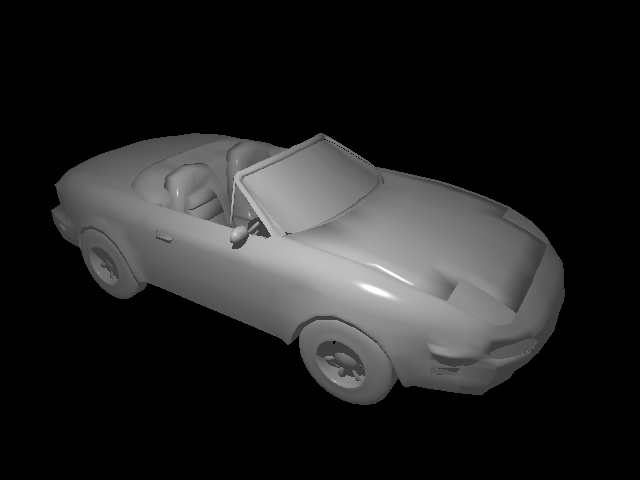
\includegraphics[width=5.5cm]{car.png}
\caption{Car model (12819 triangles)}
\end{center}
\end{figure}
\vspace{-0.5cm}

The justification for adding BVH is hopefully easy to see. After having implemented Phong
shading and lighting we naturally wanted to see the result on some more complex models,
and the poor performance became an issue. In addition, when reading about BVH and ray
tracing one gets the impression that it is quite the important part of a good
ray tracer. We did not know about this when planning the project and so did not include
it in the specification.

\subsubsection{Metallic reflection mode}
The \texttt{Material} structure has been equipped with a property for indicating that reflections
should be blended in a ''metallic mode'', which is to say that the reflected image should
be heavily tinted by the color of the reflective material. The raytracer was then extended
to handle such materials by computing a grayscale conversion (by RGB average) of the reflected
color and multiplying it by the diffuse base color of the reflective material. This method
has, as far as we know, no real basis in physics, but it works quite well to produce the desired
effect. The idea for the metallic reflection mode came after having changed to per-channel
reflectivity and having trouble trying to make a metallic material.

There is not much justification for including this feature, except that it was extremely
quick to implement.

\subsubsection{Lua scripting}
Lua scripting support has been added to the main application. Upon pressing the
F5 key, the program will try to load and run the file ''script.lua''. Pressing
the key a second time will reset the Lua environment and re-run the file. It is also possible
to select a new filename for loading with the F5 key by pressing the F key and selecting a new
\texttt{.LUA} file in the file dialog. The following
list describes what can be controlled from the script environment:

\begin{itemize}
\item Clearing the scene, removing all lights, objects, materials and textures
\vspace{-.3cm}
\item Setting the ambient light power of the scene
\vspace{-.3cm}
\item Setting the focal length, position, pitch and yaw of the camera
\vspace{-.3cm}
\item Adding and positioning lights, plus setting diffuse and specular powers
\vspace{-.3cm}
\item Loading textures
\vspace{-.3cm}
\item Adding materials and setting material properties
\vspace{-.3cm}
\item Adding spheres defined by position, radius and material
\vspace{-.3cm}
\item Building meshes by constructing triangles
\vspace{-.3cm}
\item Loading an .OBJ or .STL model, optionally applying a material to it
\vspace{-.3cm}
\item Rendering a single frame using the raytracer
\vspace{-.3cm}
\item Saving a screenshot
\end{itemize}

The Lua scripts can be thought of as the native file format for our raytracer,
capable of storing a complete scene. Now, Lua being a turing-complete programming language
this becomes quite an interesting file format, for example being capable of storing
mathematically generated structures by simply writing a Lua program to generate the structure,
including parameters for controlling the generator.
In addition, the fact that Lua is able to request a single-frame render as well as saving
a screenshot means we can render frame-by-frame animations.

The justification for adding Lua scripting is that we grew tired of editing the source
code and recompiling just to, for example, increase the power of a light source in a test
scene. The script support was added in a single afternoon and makes the program feel
much more usable.

\subsection{Missing features}
This section lists the planned features that did not make it into the project
along with short explanations for each missing feature.

\subsubsection{Area lights}
Due to the time constraints the implementation of area lights was never started.
This could have been avoided with better planning, but we could also argue that
the BVH feature is sophisticated and important enough to be a reasonable replacement.

\subsubsection{Missing bonus features}
None of the bonus features mentioned in the specification were implemented. The reason
for this is likely to be that we treated them as not being required, while the bonus
features that ended up being implemented were either out of necessity or just a quick addition.

\section{Evaluation}
Unfortunately we ran out of time while trying to create the planned comparison images. Alot
of time was wasted trying to get hold of a Stanford bunny with precomputed vertex normals.
We should obviously have started working on the comparison images much earlier.

\section{Discussion/Reflection}
\subsection{What did we learn?}
\textbf{Mikael:}
\begin{quote}
Besides what was learned from the labs and learning an awful lot of C++ during the project,
I've learned about how simple it is (mathematically) to generate really incredible images
using raytracing. More specifically, things that were new to me were ray-sphere intersections,
barycentric coordinates and their applications for texture mapping (I did texture mapping as
an experiment for lab 3 without barycentric coordinates, instead using the screen-space
interpolation of vertex properties) and Phong interpolation. Also new were the full details
of the combination of Phong interpolation and Phong illumination, and I've learned while
researching that these days people are using less of Phong and more of a topic called BRDF,
and that raytracing in general is moving (or has moved already) to more rigorously
physically-based models and path tracing.
I've also learned that raytracing without some form of search-space reduction is painfully
slow, even on modern machines, and I've come up with a simple algorithm (surely a reinvention)
for computing a BVH. Also new was the separating axis theorem and its use for triangle-box
intersection, spherical texture coordinates, the .OBJ and .STL formats, and multithreading
in C/C++ using pthreads.
\end{quote}
\bigskip
\textbf{Robin:}
\begin{quote}
I've learned that I actually can code. No really, I've always thought that I needed help to do 
any coding at all but I see now that I can do it on my own. 
I've learned that raytracing is very straight forward, and I guess it should be since it's 
a digital interpretation of what happens in real life. I've also learned alot about reflection, 
refraction, alpha blending, stl format and BVH. Even though we didn't have time to implement 
normal mapping I've read up quite a bit about it and learned a lot about that too. 
If raytracing was faster, we'd have alot better looking computer games.
This project has left me crawing more improvements for raytracing and I'll probably tinker a whole
lot on this project over the summer.
\end{quote}

\subsection{Ideas for improvements}
\subsubsection{Reducing branching in raycasting function}
Support for texture mapping added three new branches in the performance-critical raycasting
function. An improvement could potentially be made by always performing the multiplication
of base and texture colors and having materials be initialized with mock texture
objects that simply return $(1,1,1)$ on calls to \texttt{getColorAt()}.

\subsubsection{Proper handling of pixel formats in SDLTexture}
\texttt{SDLTexture} currently assumes that the image data (loaded by \texttt{SDL\_image}) is in the
\texttt{RGBA8888} format. For many formats and files this is not the case, and scenes using such files
for textures will not render correctly.

\subsubsection{Access to methods for dealing with problematic normals when loading models in Lua scripts}
Lua scripts are currently not able to specify a \texttt{VertexOrder} when loading models and is
also not able call any of the various methods that are available for dealing with problematic model
files such as \texttt{Mesh::flipY} and \texttt{Mesh::flipNormals}. These features were used quite heavily
when testing by editing the source code directly, and it is a shame they were not exposed to lua
in time for the deadline.

\subsubsection{Object translation, rotation and scaling in Lua scripts}
There is currently no support for translating, rotating or scaling an object from the
Lua environment. Since scripts can be used to create animations, being able to move
and rotate objects would be a useful improvement.

\section{References}
Please refer to the footnotes for references.

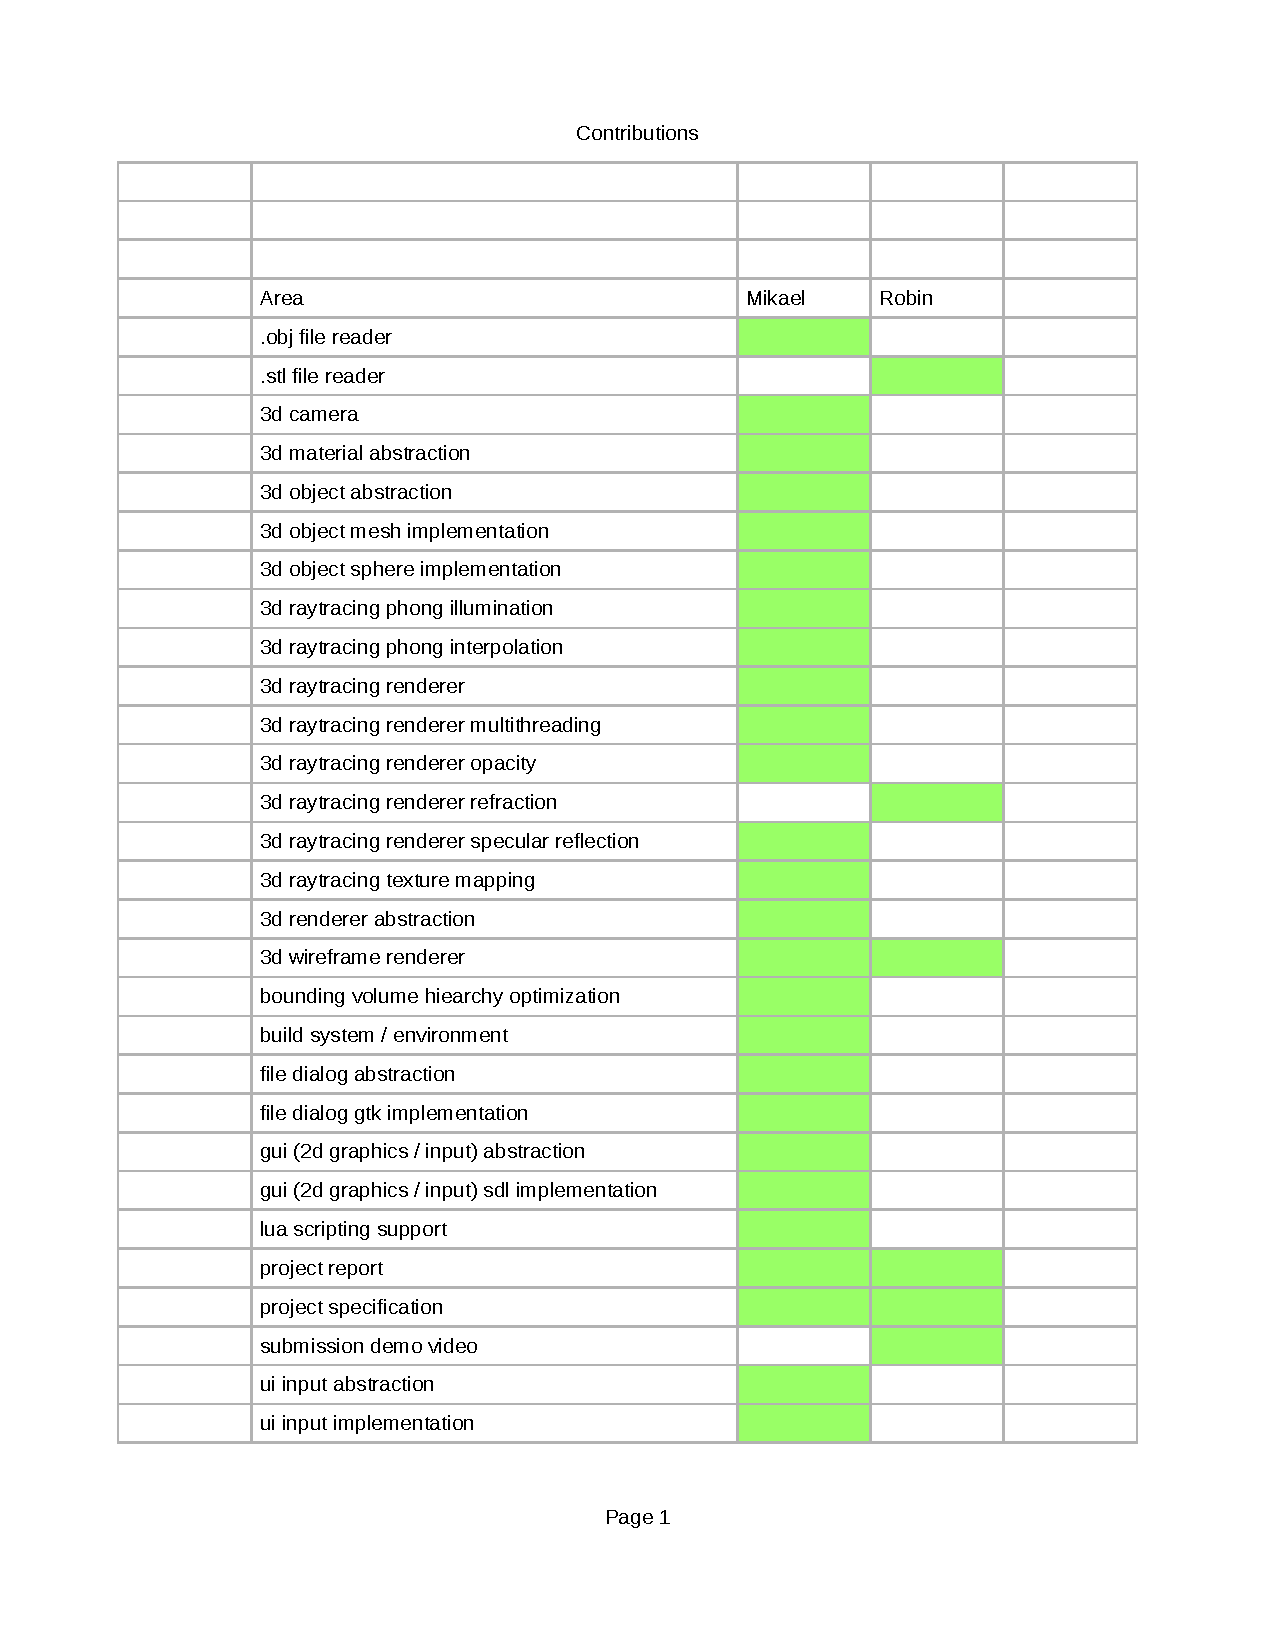
\includepdf{../contributions.pdf}
\end{document}
